\documentclass[12pt, a4paper, titlepage]{article}

\usepackage{authblk}
\usepackage{siunitx}
\usepackage{graphics}
\usepackage{subcaption}
\usepackage{tikz}
\usepackage{color}
\usepackage{lineno}
\usepackage{hyperref}
\hypersetup{
	colorlinks,
	linktoc=all,
	citecolor=blue,
	filecolor=black,
	linkcolor=black,
	urlcolor=blue
}

\begin{document}
% -------------------------------------------------------------------------------------
% TITLE PAGE
% -------------------------------------------------------------------------------------
\begin{titlepage}
	\centering
	
\includegraphics[scale=0.3]{figures/KIT-logo.png} \\
	\vspace{2cm}
	{\huge\bfseries McCAD v1.0\par}
	\vspace{1.5cm}
	{\Large\itshape Moataz Harb\\moataz.harb@kit.edu\par}
	\vspace{1cm}
	{\Large\itshape Karlsruhe Institute of Technology (KIT), Hermann-von-Helmholtz-Platz 1, 76344 Eggenstein-Leopoldshafen, Germany\par}
	\vfill
	% Bottom of the page
	{\large \today\par}
\end{titlepage}
\clearpage

% -------------------------------------------------------------------------------------
% TABLE OF CONTENTS
% -------------------------------------------------------------------------------------
\tableofcontents
\clearpage

% -------------------------------------------------------------------------------------
% INTRODUCTION
% -------------------------------------------------------------------------------------
\section{Introduction} \label{sec:Introduction}
McCAD is a library with an executable for the conversion of CAD solid models to the input syntax of the Monte Carlo (MC) code MCNP; from Boundary Representation "BREP" to Constructive Solid Geometry "CSG". The library is written in C++ and uses CMake as a build system. It has Open CASCADE Technology and Boost C++ libraries as dependencies. Currently, the library is capable of processing solids with the following surface types and their combinations:
\begin{itemize}
	\item planar
	\item cylindrical
	\item toroidal
         \item conical
\end{itemize}
The general capabilities/output of the library include:
\begin{itemize}
	\item producing a list of volumes of CAD solids as loaded from the input STEP file(s).
	\item decomposing complex solids into their constituent convex primitives.
	\item converting decomposed solids into the input syntax the MC code MCNP.
	\item void generation.
	\item generating entries, surface source and cell tallies, to calculate stochastic cell volumes on the generated MC input file.
	\item producing a mapping of cell IDs on the generated MC input file to the corresponding volumes and names of CAD solids as loaded from the decomposed STEP file(s).
	\item producing a mapping of void-to-material cells in the generated MC input file.
\end{itemize}

% -------------------------------------------------------------------------------------
% Installation
% -------------------------------------------------------------------------------------
\section{Installation from Source} \label{sec:Installation from Source}
Building of the McCAD library is supported on both Linux and Windows operating systems (OS). The library has three 3rd-party dependencies: CMake, Boost C++ libraries, and Open CASCADE Technology. CMake is the standard build system for McCAD and it comes by default with most Linux distributions as well as Windows OS. Boost C++ libraries consist of header files that are utilized for parallel processing in McCAD. Open CASCADE Technology (OCCT) is used as a geometry engine for geometrical solids manipulation and decomposition. Below are guiding steps for installation on both Linux and Windows OSs. 
  \subsection{Linux}
    Listed below are the currently supported Linux distributions:
    \begin{itemize}
  	  \item Ubuntu 20.04 LTS
  	  \item Ubuntu 18.04 LTS
    \end{itemize} 
    Testing of installation on other distributions is still underway! thus Ubuntu is recommended as a distribution to install McCAD. Below are general steps to install McCAD and its dependencies.
    \begin{itemize}
  	  \item \textbf{CMake}
  	  \begin{itemize}
		\item download cmake-3.23.0.tar.gz from \url{https://cmake.org/download/} then execute the commands below in a terminal.
		\item \$ tar -xzvf cmake-3.23.0.tar.gz
		\item \$ cd cmake-3.23.0
		\item \$ mkdir build
		\item \$ cd build
		\item \$ cmake .. -DCMAKE\_USE\_OPENSSL=OFF \\-DCMAKE\_INSTALL\_PREFIX=.
		\item \$ make
		\item \$ make install
  	  \end{itemize}
      \item \textbf{Boost C++ libraries}
      \begin{itemize}
    	\item download boost\_1\_78\_0.tar.gz from \url{https://www.boost.org/users/download/} then execute the commands below in a terminal.
    	\item \$ tar -xvzf boost\_1\_78\_0.tar.gz
    	\item \emph{NOTE}: If Boost libraries are not needed for other applications, then you can skip the remaining steps!
    	\item \$ cd boost\_1\_78\_0
    	\item \$ mkdir build
    	\item \$ cd tools/build
    	\item \$ ./bootstrap.sh
    	\item \$ ./b2 install -\--prefix=../../build/
      \end{itemize}
      \item \textbf{Open CASCADE Technology (OCCT)}
      \begin{itemize}
        \item \emph{NOTE}: the instructions on the installation of dependencies can be found on the side menu in \url{https://dev.opencascade.org/doc/occt-7.5.0/overview/html/index.html} by navigating to "Build, Debug and Upgrade $>$ Build 3rd-parties" then following the instructions under "Installation from Official Repositories".
    	\item download opencascade-7.5.0.tgz from \url{https://dev.opencascade.org/release/previous} then execute the commands below in a terminal.
    	\item \$ tar -xzvf opencascade-7.5.0.tgz
    	\item \$ cd opencascade-7.5.0
    	\item \$ mkdir build
    	\item \$ cd build
    	\item \$ cmake .. -DCMAKE\_BUILD\_TYPE=Release \\-DBUILD\_LIBRARY\_TYPE=Shared \\-DCMAKE\_INSTALL\_PREFIX=. \\-DINSTALL\_TEST\_CASES=true \\-DINSTALL\_DOC\_Overview=true
    	\item \$ make
    	\item \$ make install
      \end{itemize}
	  \item \textbf{McCAD}
	  \begin{itemize}
		\item \emph{NOTE}: building a shared library is recommended! Should a static library be needed, the user has to ensure a compliant build of Open CASCADE Technology by changing "Shared" to "Static" in the build type; -DBUILD\_LIBRARY\_TYPE=STATIC.
		\item \$ git clone \url{https://github.com/inr-kit/McCAD_Library}
		\item \$ cd McCAD\_Library
		\item \$ mkdir build
		\item \$ cd build
		\item to build a shared library (\emph{recommended}):
		  \begin{itemize}
			\item \$ CMake .. \\-DCMAKE\_INSTALL\_PREFIX=. \\-DBUILD\_RPATH=true \\-DBUILD\_SHARED=true \\-DBUILD\_SHARED\_EXE=true \\-DBOOST\_CUSTOM\_ROOT=$<$Path to boost\_1\_78\_0$>$ \\-DOCC\_CUSTOM\_ROOT=$<$Path to opencascade-7.5.0/build$>$ 
			\\-DCMAKE\_EXE\_LINKER\_FLAGS="-m64 -fPIC" \\ -DCMAKE\_CXX\_FLAGS="-fPIC"
		  \end{itemize}
		\item to building a static library:
		\begin{itemize}
			\item replace "SHARED" by "STATIC" in "\\-DBUILD\_SHARED \\-DBUILD\_SHARED\_EXE in the above commands.
		\end{itemize}
		\item \$ make
		\item \$ make install
		\item add the absolute path to McCAD/build/bin to .bashrc file or create an alias for McCAD to run from command line.
	  \end{itemize}
    \end{itemize}

  \subsection{Windows}
    Listed below are the currently supported Windows versions (testing of installation on other versions is still underway!):
    \begin{itemize}
  	  \item Windows 10
    \end{itemize} 
    Below are the general steps to build McCAD library and its dependencies.
    \begin{itemize}
	  \item \textbf{CMake} (optional)
 	  \begin{itemize}
    	\item \emph{NOTE}: If usage of IDE - such Microsoft Visual Studio (VS) - is intended, then installing CMake can be skipped since most IDE builds CMake by default. However, it is recommended to update CMake and adding the full path to the bin folder to the "Path" environment variable.
 		\item download and run the installer cmake-3.23.1-windows-x86\_64.msi from \url{https://cmake.org/download/}.
  	  \end{itemize}
	  \item \textbf{Microsoft Visual Studio}
	  \begin{itemize}
		\item download the "community" installer (version 17 2022) from \\\url{https://visualstudio.microsoft.com/downloads/}.
		\item run the installer and make sure to enable "Desktop development with C++" on the main menu and ""Windows 10 SDK" on the side menu under "Desktop development with C++".
	  \end{itemize}
      \item \textbf{Boost C++ libraries}
      \begin{itemize}
    	\item download boost\_1\_78\_0.zip from \url{https://www.boost.org/users/download/}.
    	\item unzip boost\_1\_78\_0.zip.
    	\item \emph{NOTE}: if boost will be used for other applications then you can check the documentation in index.html in the unzipped folder for instruction on building the library. Otherwise, no need to build the library since McCAD only uses the header files.
      \end{itemize}
      \item \textbf{Open CASCADE Technology (OCCT)}
	  \begin{itemize}
		\item download and run the installer opencascade-7.5.0-vc14-64.exe from \url{https://dev.opencascade.org/release/previous}.
		\item after successful installation there will be different folders for the many toolkits that come with a full installation of opencascade; such as freeimage, ffmpeg, openvr, vtk, etc. It is recommended to add the full path to all bin folders to the Windows "Path" environment variable.
	  \end{itemize}
	  \item \textbf{McCAD}
	  \begin{itemize}
	  	\item It is recommended to restart the PC/Laptop before proceeding to allow the changes to the "Path" environment from above to take effect. 
		\item download, by selecting "Code $>$ Download ZIP", source code from \\\url{https://github.com/inr-kit/McCAD-Library}.
		\item unzip McCAD\_Library.
		\item open MSVC and select the McCAD\_Library folder.
		\item from the "Solution Explorer - Folder Review" double click CMakeSettings.json file. This will open the file in IDE. \item Set a "Configuration name". 
		\item ensure that "Configuration type" is set to "Release" and "Toolset" is set to "msvc\_x64\_x64".
		\item to build a static library (\emph{recommended}):
		  \begin{itemize}
		  	\item ensure that the following is on "CMake command arguments" \\-DLINUX\_OS=false \\-DBUILD\_RPATH=true \\-DBUILD\_STATIC=true \\-DBUILD\_STATIC\_EXE=true \\-DBOOST\_CUSTOM\_ROOT="$<$Path to boost\_1\_78\_0$>$" \\-DOCC\_CUSTOM\_ROOT="$<$Path to OpenCASCADE-7.5.0-vc14-64\textbackslash opencascade-7.5.0$>$"
		  \end{itemize}
		\item to build a shared library:
		\begin{itemize}
			\item replace the word "STATIC" by "SHARED" in \\-DBUILD\_STATIC \\-DBUILD\_STATIC\_EXE in the above commands.
		\end{itemize}
		\item from the top menu select "Build $>$ Build All".
		\item after successful completion of the previous step, from the top menu select "Build $>$ Install McCAD".
		\item add the full path to McCAD\_Library/build/bin to the PATH environment variable. 
	  \end{itemize}
    \end{itemize}

% -------------------------------------------------------------------------------------
% I/O
% -------------------------------------------------------------------------------------
\section{I/O} \label{sec:I/O}
In general, there are three types of information that need to be provided to McCAD: geometry model(s), materials assignment, and running parameters. Below, the input pertinent to the decomposition and conversion will be highlighted. The output from McCAD will depend on the mode of execution, as will be described in the following sections.
  \subsection{General}
	The first input to be provided is the input configuration file, McCADInputConfig.i.  When run via a command line \emph{without arguments}, McCAD will generate a template configuration file, figure (\ref{fig:config}), with the default values of the run parameters. In both run modes, decomposition and conversion, McCAD input parameters are needed. The run parameters are assigned values by default and can be modified by the user. Below is a description of the general input parameters.
	\begin{figure}[h!]
		\centering
		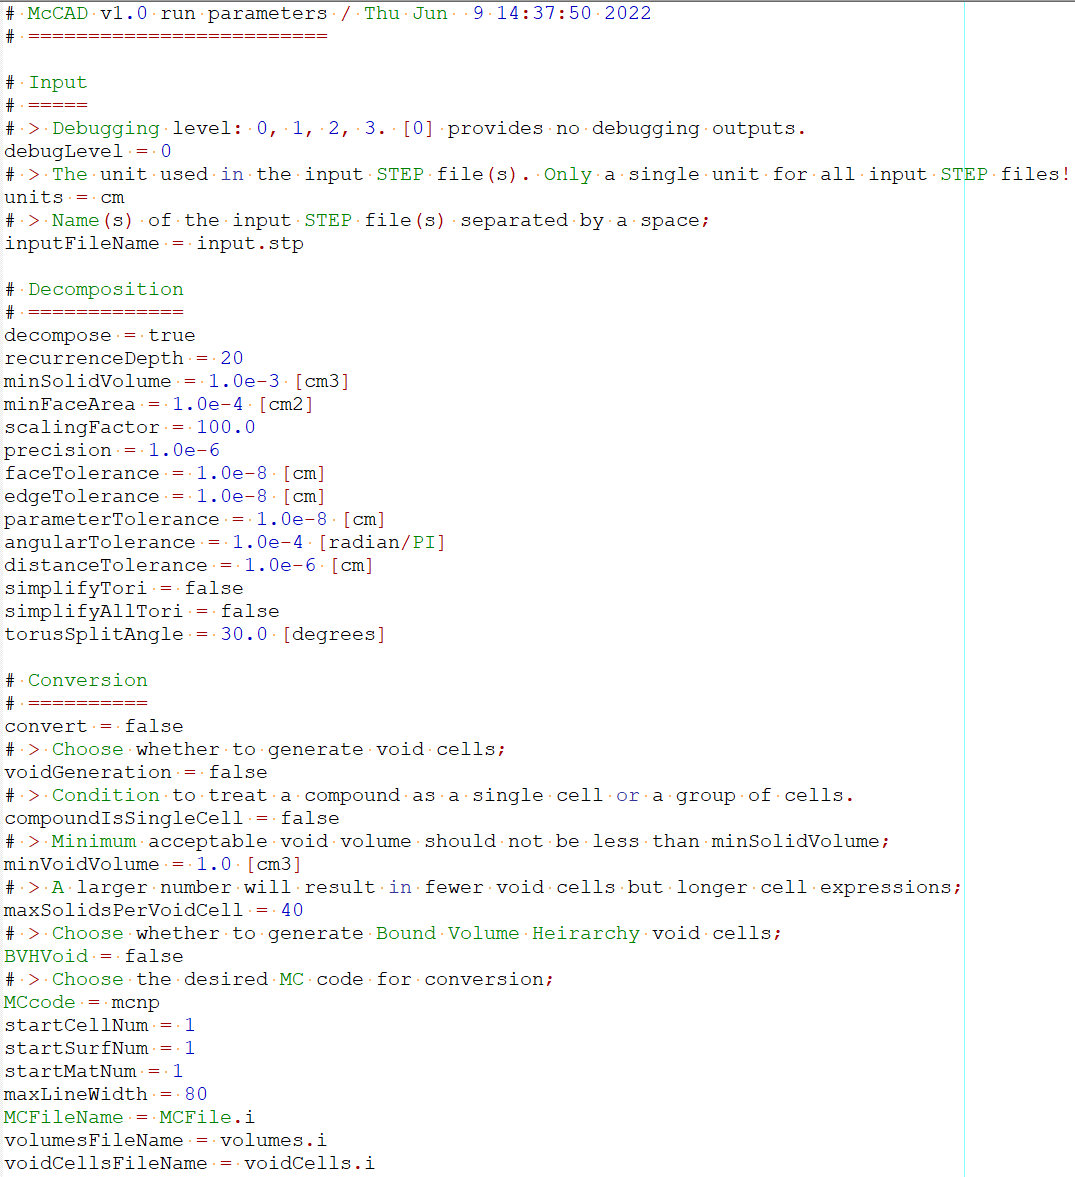
\includegraphics[scale=0.5]{figures/configFile.png}
		\caption{McCAD Input Configuration File}
		\label{fig:config}
	\end{figure}
	\begin{itemize}
		\item \textbf{debugLevel}: the level at which run/debug info is displayed on the screen. \emph{Default} is 0.
		\item \textbf{units}: the units used in the CAD model. \emph{Default} is cm.
		\item \textbf{inputFileName}: the input STEP file(s) name(s). \emph{Default} is input.stp.
	\end{itemize}

  \subsection{Decomposition}
    Currently McCAD supports input files in the STEP format (protocol 214). McCAD accepts both single and multiple input STEP files. For each input STEP file, after successfully running McCAD decomposition two STEP output files will be written to disk. The first will contain the decomposed input solids and the second will contain the rejected/failed input solids. If the latter is absent, this means no input solids were rejected and no solids failed to be decomposed. \\
    \\
    Before running McCAD in the decomposition mode, the user is advised to review the input parameters on the decomposition section on the input configuration file, figure (\ref{fig:config}). Below is a description of the decomposition input parameters.
	\begin{itemize}
	  \item \textbf{decompose}: a logical condition for running decomposition on the input file(s). \emph{Default} is true.
	  \item \textbf{recurrenceDepth}: defines the level of decomposition performed recursively on input solids. This input specifies the maximum number of recursive application of decomposition on the subsolids. The larger the number, the less the failed solids. \emph{Default} is 20.
	  \item \textbf{minSolidVolume}: controls the recursive splitting of the solids along with the recurrenceDepth. It is also used to filter out the input solids by rejecting solids with smaller volumes than the specified value. \emph{Default} is 10\textsuperscript{-3} cm\textsuperscript{3}.
	  \item \textbf{minFaceArea}: used to filter out the input solids by rejecting solids with faces smaller in area than the specified value. \emph{Default} is 10\textsuperscript{-4} cm\textsuperscript{2}.
	  \item \textbf{scalingFactor}: controls the size of generated mesh on solid faces. This parameter mainly affects the collision detection of surfaces. More details can be found in section \ref{sec:Theory of McCAD Conversion}. \emph{Default} is 100.0.
	  \item \textbf{precision}: used to judge the equality of numerical values. \emph{Default} is 10\textsuperscript{-6}.
	  \item \textbf{faceTolerance}: more details can be found in section \ref{sec:Theory of McCAD Conversion}. \emph{Default} is 10\textsuperscript{-8} cm.
	  \item \textbf{edgeTolerance}: more details can be found in section \ref{sec:Theory of McCAD Conversion}. \emph{Default} is 10\textsuperscript{-8} cm.
	  \item \textbf{parameterTolerance}: more details can be found in section \ref{sec:Theory of McCAD Conversion}. \emph{Default} is 10\textsuperscript{-8} cm.
	  \item \textbf{angularTolerance}: more details can be found in section \ref{sec:Theory of McCAD Conversion}. \emph{Default} is 10\textsuperscript{-4} radian/PI.
	  \item \textbf{distanceTolerance}: more details can be found in section \ref{sec:Theory of McCAD Conversion}. \emph{Default} is 10\textsuperscript{-6} cm.
	  \item \textbf{simplifyTori}: a logical condition on whether to simplify toroidal solids as a collection of smaller cylindrical segments. If \emph{true}, only off axis tori will be simplified. \emph{Default} is false.
	  \item \textbf{simplifyAllTori}: a logical condition on whether to simplify all toroidal solids as a collection of smaller cylindrical segments. If \emph{true}, all toroidal solids, disregarding its axis, will be simplified. \emph{Default} is false.
	  \item \textbf{torusSplitAngle}: the angle between the top and bottom bases of a cylindrical segment. The angle controls the number of cylindrical segments the torus is simplified to. \emph{Default} is 30.0 degrees.
    \end{itemize}

  \subsection{Conversion}
    McCAD conversion will result in three textual output files. The first contains the generated MC, MCNP is only support for now, input file. The second contains a mapping of cell ID, volume, and solid name. The third file contains a mapping of void-to-material cell IDs. More details on the format of the three files can be found in section \ref{sec:Example}. \\
    \\
    Material assignment is currently deduced from the name of the input STEP file(s). The user is advised to split the CAD model into several by material. The name of the input STEP files takes the format $<$material name$>$\_$<$density in exponential format: -0.0E0$>$\_$<$.stp. The material name and density are then extracted from the file name and assigned to the solids it contains. For MCNP, the sign of the density implies whether mass or atomic densities is used. In case of absence of the density value, void is assumed. It is important to note that the underscore occurs once in the file name and only separates the material name from density. Any extra underscores will result in an error. \\
    \\
    Before running McCAD in the conversion mode, the user is advised to review the input parameters on the conversion section on the input configuration file, figure (\ref{fig:config}). Below is a description of the conversion input parameters.
	\begin{itemize}
	  \item \textbf{convert}: a logical condition for running conversion on the input file(s). \emph{Default} is false.
	  \item \textbf{voidGeneration}: a logical condition for void generation. If false, only a single void cell is created outside which is a graveyard. \emph{Default} is false.
	  \item \textbf{compoundIsSingleCell}: controls whether to define the subsolids of the decomposed input solid into separate cells or unify it through the union operator into a single cell. If \emph{true}, all subsolids are joined  through a union operator and a single cell is written to the MC input file. This is not recommended for complex solids since it slows down the transport due to the many surface crossing checks. \emph{Default} is false.
	  \item \textbf{minVoidVolume}: controls the desirable minimum void cell volume. \emph{Default} is 1.0 cm\textsuperscript{3}.
	  \item \textbf{maxSolidsPerVoidCell}: controls the number of generated void cells. A smaller number will result in a larger number of void cells each with simpler expression on the MC file. \emph{Default} is 40.
	  \item \textbf{BVHVoid}: a logical condition for generating a bound volume hierarchy void cells. This feature is still undergoing testing and not currently recommended to be used. \emph{Default} is false.
	  \item \textbf{MCcode}: specifies the targeted MC code to generate the input file in a compliant format. Currently only MCNP is supported. \emph{Default} is mcnp.
	  \item \textbf{startCellNum}: the desired starting cell number. \emph{Default} is 1.
	  \item \textbf{startSurfNum}: the desired starting surface number. \emph{Default} is 1.
	  \item \textbf{startMatNum}: the desired starting material number. \emph{Default} is 1.
	  \item \textbf{maxLineWidth}: maximum length of lines on the MC file. \emph{Default} is 80.
	  \item \textbf{MCFileName}: the desired name for the MC file. \emph{Default} is MCFile.i.
	  \item \textbf{volumesFileName}: the desired name for the cell ID-volumes-name mapping file. \emph{Default} is volumes.i.
	  \item \textbf{voidCellsFileName}: the desired name of the void to material cells mapping file. \emph{Default} is voidCells.i.
    \end{itemize}

% -------------------------------------------------------------------------------------
% Running McCAD
% -------------------------------------------------------------------------------------
\section{Running McCAD} \label{sec:Running McCAD}
There are two ways to run McCAD, via a command line or the SpaceClaim plugin. McCAD can be run from a command line either in a Linux terminal or a Windows command prompt.

  \subsection{Command Line}
    On a Linux terminal or Windows command prompt McCAD can be run by typing in the path to the executable followed by the desired argument. A good practice is to add the full path of the McCAD executable to the PATH environment variable then simply call "McCAD" with the acceptable desired command line arguments. The arguments could be displayed on the screen by running "McCAD help". The acceptable McCAD arguments are listed below.
    \begin{itemize}
      \item \textbf{[]}: running McCAD without arguments will result in writing McCAD template input configuration file, McCADInputConfig.i.
      \item \textbf{[help]}: lists all the acceptable arguments.
      \item \textbf{[read]}: test loading the solids from the input STEP file(s). This is used to test if the OCCT reader will fail to load any STEP file(s). McCAD will generate a text file per input STEP file that contains the volumes of shapes contained in the file.
      \item \textbf{[run]}: executes McCAD according to the selected running mode on the McCADInputConfig.i file; decomposition, conversion, or both. 
    \end{itemize}

  \subsection{SpaceClaim Plugin}
    The python script located in plugins/SpaceClaim\_interface can be loaded into SpaceClaim and used directly to call McCAD to perform decomposition on selected solid(s).  The script can be loaded in SpaceClaim by selecting "File $>$ New $>$ Script". Select the desired solid(s) to decompose and on the "Script Editor" select "Run Script", the green arrow.
    \\\\
    Figure (\ref{fig:SCPlugin}) shows a screen shot from a loaded script in SpaceClaim. After loading the script into SpaceClaim, the user should modify \emph{McCADExecutable} and \emph{workPath} variables according. The former should be modifyied to point to McCAD executable that will be called by the script. The latter is the desired work directory that the temporary files will be created in. The user then can select solid(s) from the model and run the plugin using the green arrow at the top right corner. After running McCAD, a summary will be printed in the "Interpreter" as shown at the bottom of figure (\ref{fig:SCPlugin}).
    \\\\
    If the user which to modify the input configuration file, McCADInputConfig.i, there are two way to do so. The first is to copy the template from the templates folder and place it in the "workPath" folder. Another way is by running the script without selecting any solids. This way McCAD will generate the McCADInputConfig.i file which the user can modify.
    \begin{figure}[h!]
    	\centering
    	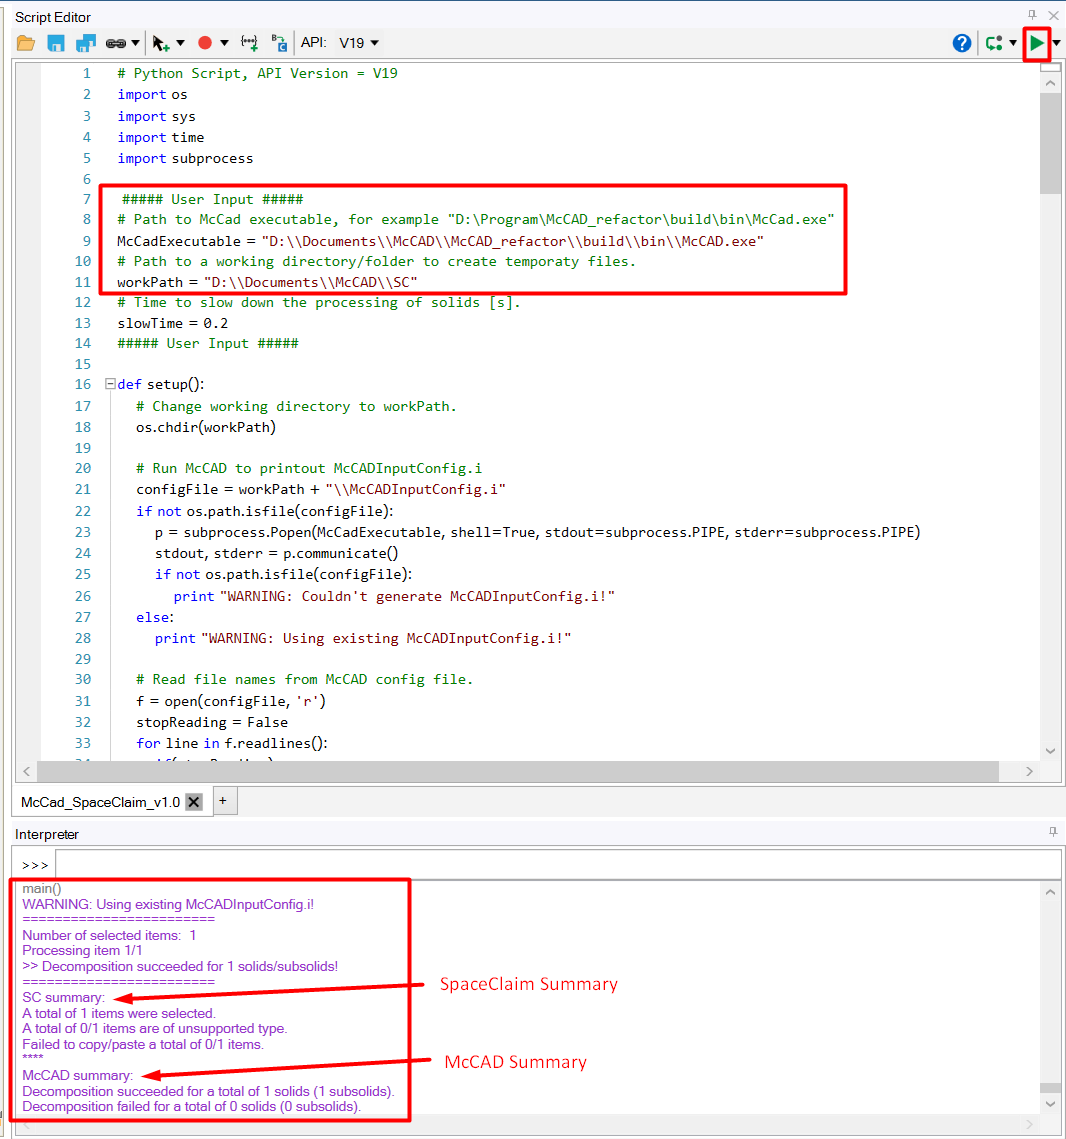
\includegraphics[scale=0.5]{figures/SC_plugin.png}
    	\caption{Example Input Solids}
    	\label{fig:SCPlugin}
    \end{figure}

% -------------------------------------------------------------------------------------
% Example
% -------------------------------------------------------------------------------------
\section{Example} \label{sec:Example}
This section will discuss how to run McCAD from a command line. The example input STEP file as well as the output files can be found in examples/collection\_of\_solids folder. The input file, SS\_-793e-2.stp, contains a collection of random solids, as shown in figure (\ref{fig:ExampleSolids}); with steps, cylinders, tori, protrusions, depressions, etc. The solids from the file are assigned stainless steel material (SS) with a density of 7.93 g/cm\textsuperscript{3}, as indicated by the name of the STEP file.
\begin{figure}[h!]
	\centering
	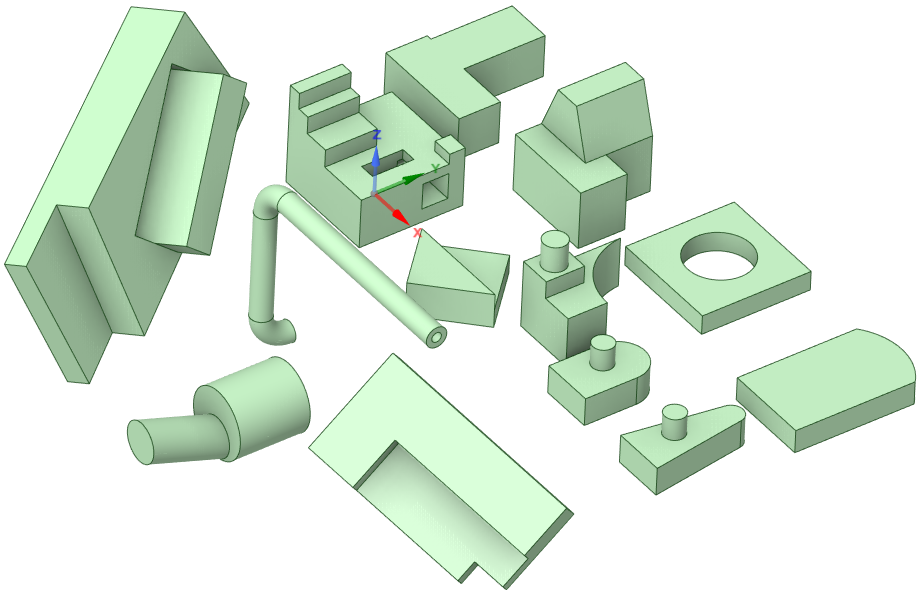
\includegraphics[scale=0.42]{figures/InputSolids.png}
	\caption{Example Input Solids}
	\label{fig:ExampleSolids}
\end{figure}

\begin{enumerate}
  \item with the path to McCAD executable added to the PATH environment variable, the McCADInputConfig.i file could be generated by running McCAD, without any arguments, figure (\ref{fig:McCAD_output}).
  \begin{figure}[h!]
  	\centering
  	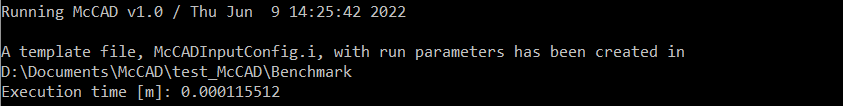
\includegraphics[scale=0.7]{figures/McCAD_output.png}
  	\caption{McCAD Displayed Output}
  	\label{fig:McCAD_output}
  \end{figure}

  \item on McCADInputConfig.i file, the \emph{inputFileName} should be changed to SS\_-793e-2.stp. Also, \emph{simplifyTori}, \emph{convert}, and \emph{voidGeneration} parameters should all be set to \emph{true}.
  
  \item McCAD is then run via the command "McCAD run". After successfully running McCAD there should be a total of five new files generated on disk. Figure (\ref{fig:McCAD Decomposition and Conversion Outputs}) shows the displayed output of McCAD on screen for decomposition and conversion.
  \begin{figure}[h!]
  	\centering
  	\begin{subfigure}{.5\textwidth}
  		\centering
  		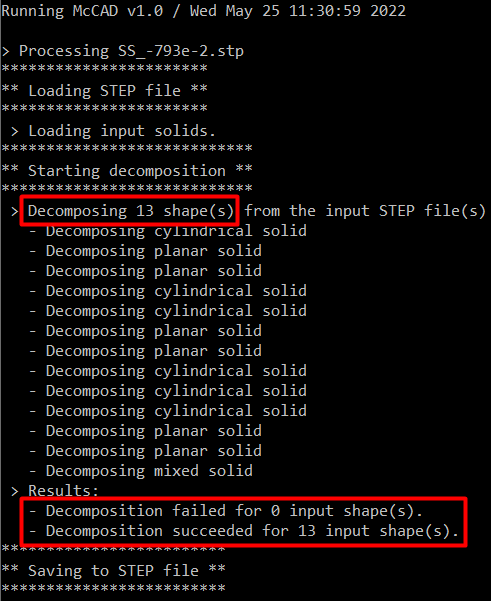
\includegraphics[width=.8\linewidth]{figures/McCAD_output_decomposition.png}
  		\caption{}
  		\label{fig:a}
  	\end{subfigure}%
  	\begin{subfigure}{.5\textwidth}
  		\centering
  		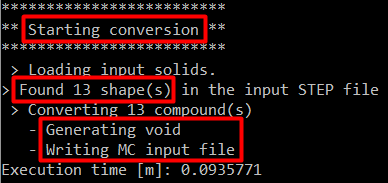
\includegraphics[width=.8\linewidth]{figures/McCAD_output_conversion.png}
  		\caption{}
  		\label{fig:b}
  	\end{subfigure}
  	\caption{McCAD Decomposition (a) and Conversion (b) Displayed Outputs}
  	\label{fig:McCAD Decomposition and Conversion Outputs}
  \end{figure}

  \begin{itemize}
  	\item the first file is produced by McCAD STEP file reading algorithm, SS\_-793e-2Volumes.i, and contains a list of solid volumes and their names as read from the input STEP file, SS\_-793e-2.stp.
  	
    \item the second file is produced by McCAD decomposition algorithm, SS\_-793e-2Decomposed.stp, and contains the decomposed input solids. Upon loading the file into any CAD software we could see the decomposed solids, as shown in figure (\ref{fig:Decomposed Solids}).
	\begin{figure}[h!]
		\centering
		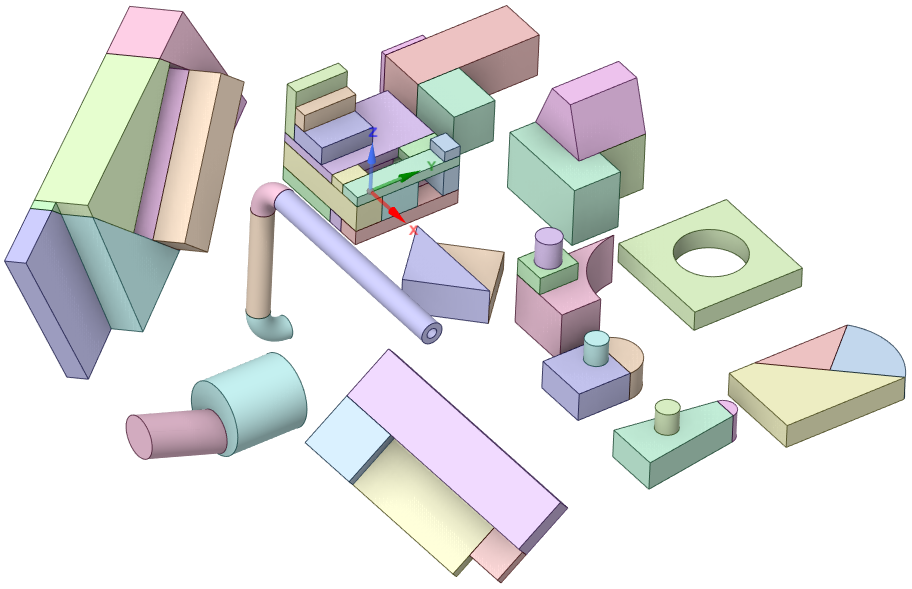
\includegraphics[scale=0.4]{figures/decomposedSolids.png}
		\caption{McCAD Decomposed Input Solids}
		\label{fig:Decomposed Solids}
	\end{figure}

	\item the third file is produced by McCAD conversion algorithm, MCFile.i. The file is the MCNP input file and contains cells, surfaces, and data cards in MCNP format, figure (\ref{fig:MCFile}).
	\begin{figure}[h!]
		\centering
		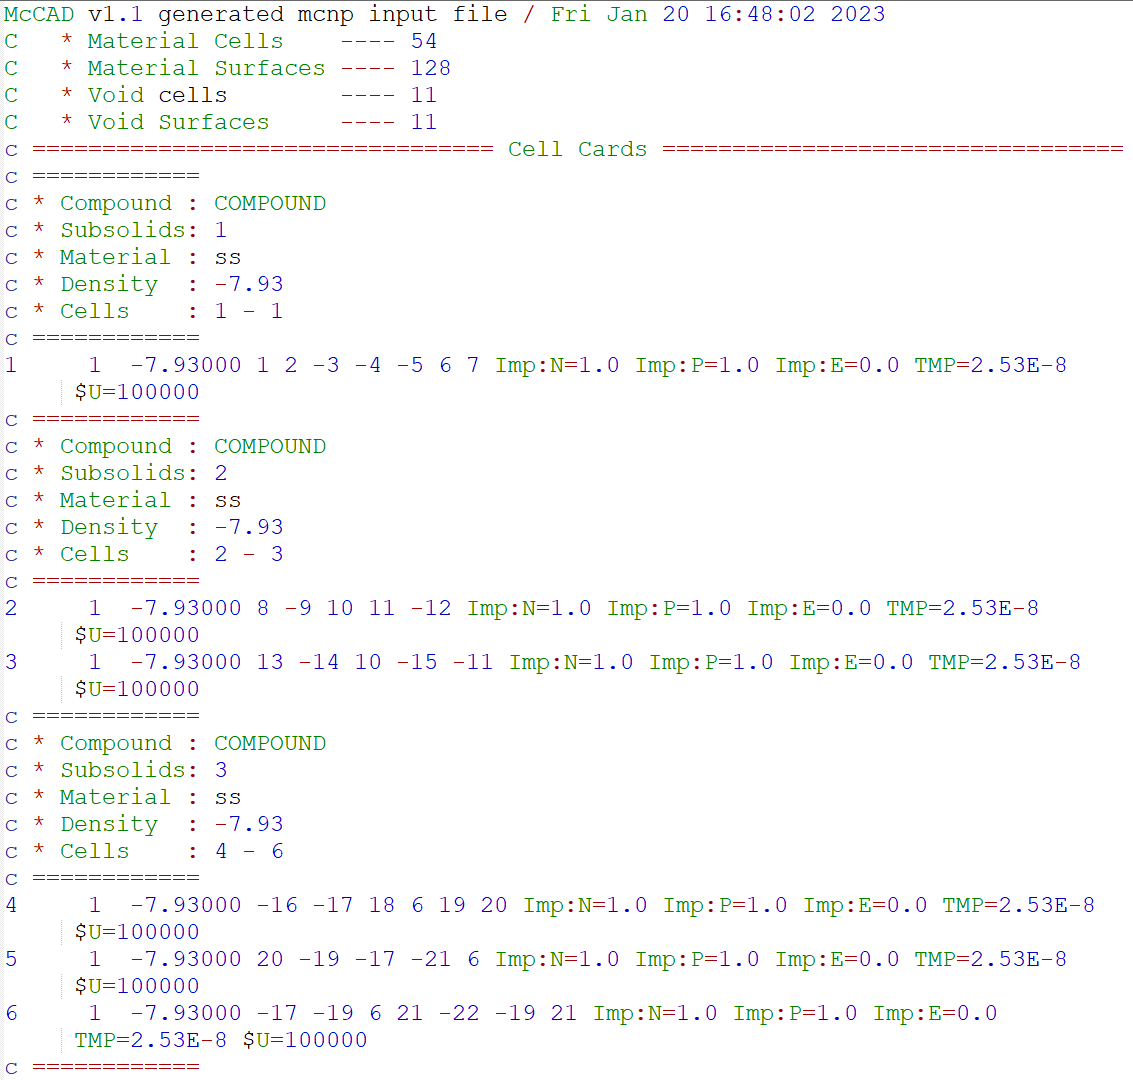
\includegraphics[scale=0.5]{figures/cellCards.png}
		\caption{McCAD Generated MCFile.i File}
		\label{fig:MCFile}
	\end{figure}

	\item the fourth file is produced by McCAD conversion algorithm, volumes.i. The file lists cell IDs, volumes of solids, and name on the CAD STEP file, figure (\ref{fig:volumes file}).
	\begin{figure}[h!]
		\centering
		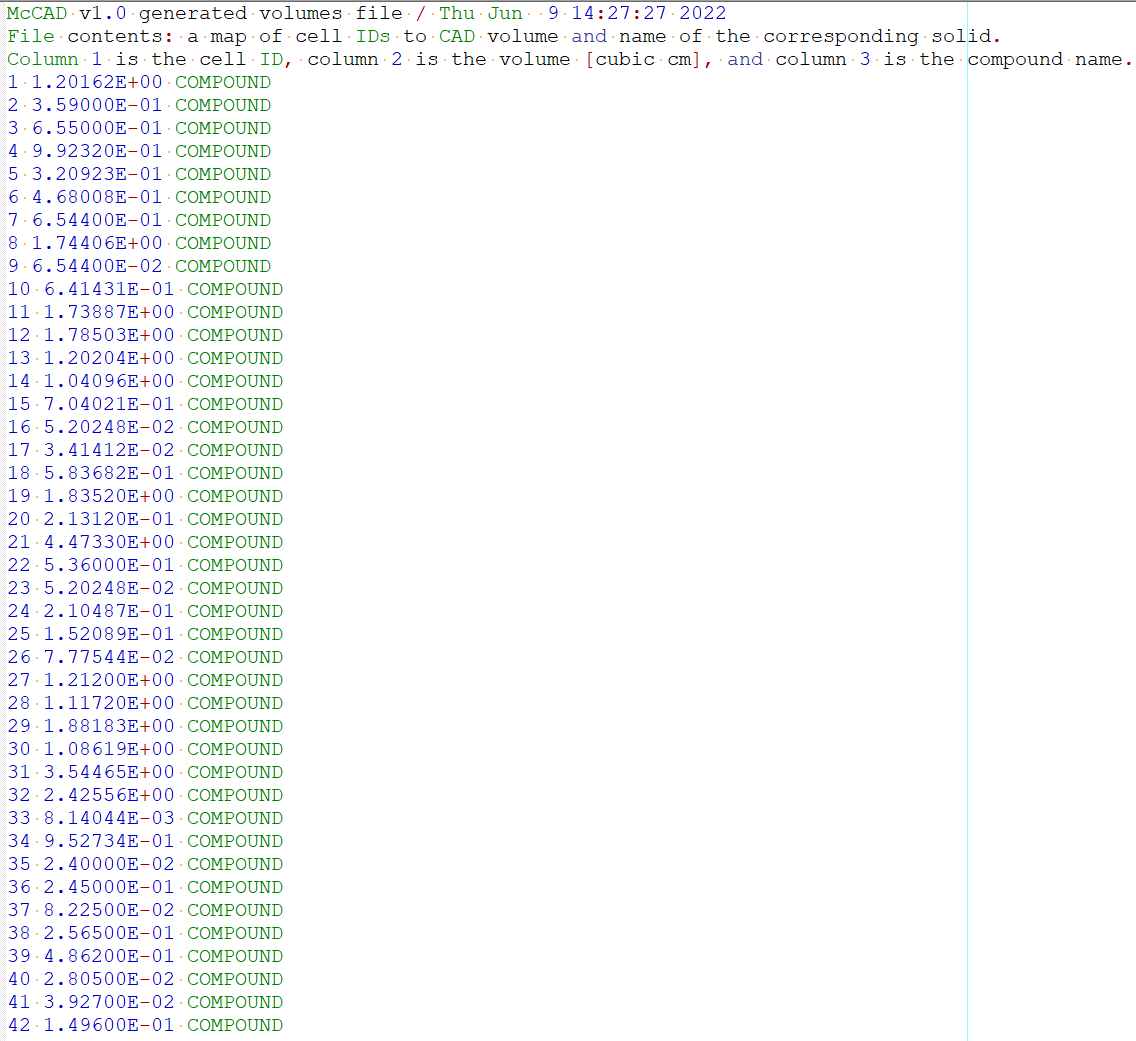
\includegraphics[scale=0.5]{figures/volumesFile.png}
		\caption{McCAD Generated volumes.i File}
		\label{fig:volumes file}
	\end{figure}

	\item the fifth file is produced by McCAD conversion algorithm, voidCells.i. The file maps void to material cell IDs, figure (\ref{fig:void cells file}).
	\begin{figure}[h!]
		\centering
		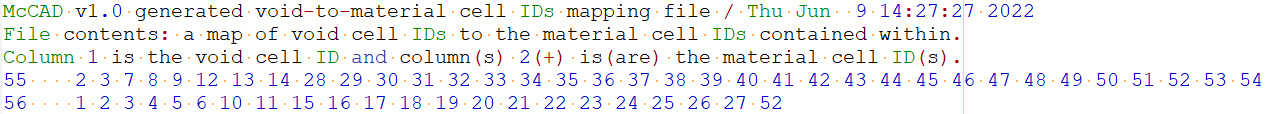
\includegraphics[scale=0.4]{figures/voidCellFile.png}
		\caption{McCAD Generated voidCells.i File}
		\label{fig:void cells file}
	\end{figure}
  \end{itemize}

  \item Using MCNP plotter, figure (\ref{fig:MCFile.i plot}) shows a plot of the MCFile.i and the corresponding CAD cross-section.
  \begin{figure}[h!]
  	\centering
  	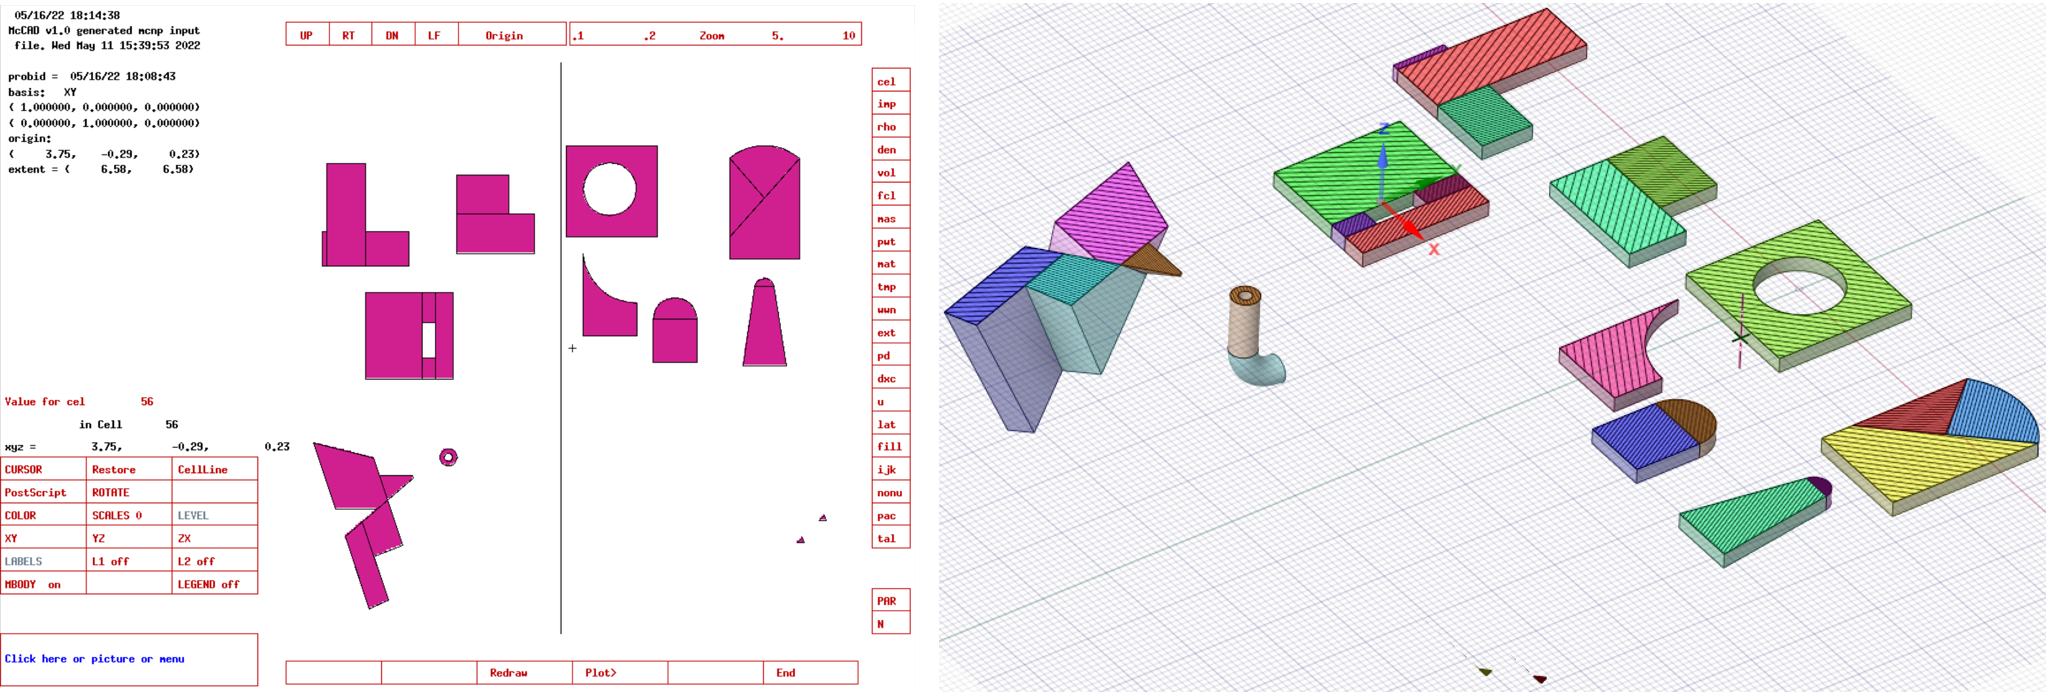
\includegraphics[scale=0.32]{figures/ConvertedSolids.png}
  	\caption{MCNP Plot of MCFile.i}
  	\label{fig:MCFile.i plot}
  \end{figure}
\end{enumerate}

% -------------------------------------------------------------------------------------
% General Usage Notes
% -------------------------------------------------------------------------------------
\section{General Usage Notes} \label{sec:General Usage Notes}
The following are general notes and best practices for using McCAD.
\begin{itemize}
	\item it is better to run decomposition and conversion separately!. This is the main reason why the conversion is disabled by default on the McCADInputConfig.i file. Checking the decomposed CAD solids for errors or interference is always advised! 
	\item a good practice is to decompose the model few solids at a time. This ensures a smoother decomposition, as well as makes it easier to locate the troubling solid or part of the model.
	\item currently, complex hollow planar solids might result in large STEP files. It is a good practice to aid the decomposition by manually cutting the solid in two, three, or more subsolids then run McCAD on the subsolids.
	\item before running the conversion, it is better to check in CAD for any interferences in the model. This is especially needed if simplification of tori is enabled. A clean model will result in a conversion with less errors.
	\item before running McCAD conversion on the entire model, test the conversion on parts of the model separately. A good practice is to convert the solids that belong to a single material together. Test converting solids with another material. Then test converting both together. This way it is much easier to trace back the source of error and correct it in CAD rather than converting the entire model and try to figure out a solution to geometry errors.
	\item if the user wants a list of the CAD volumes, McCAD conversion STEP reader produces, in joint decomposition and conversion, mode, a volumes file with the format $<$file name$>$DecomposedVolumes.i. This file represents a list of volumes of the decomposed solids that will be converted. Running mcnp to calculate the stochastic cell volumes will produce volumes per cell. This way, the user will have a quantitative measure of the deviation of solid volumes due to decomposition and conversion; an important validation measure for converted CAD models.
	\item if McCAD decomposition and conversion are run separately, it is advised to rename the original volumes file so as not to get not overwritten by the volumes file produced by the conversion run. This way the user will have volumes file for the original solids as well as for the solids after decomposition.
\end{itemize}

% -------------------------------------------------------------------------------------
% Knows Issues
% -------------------------------------------------------------------------------------
\section{Known Issues} \label{sec:Known Issues}
Through extensive testing of McCAD decomposition and conversion core algorithms, some issues were found in relation to processing of solids. While some issues were fixed, not reported here, through debugging others persist and are in line to be addressed. Below is a list of the current known issues and how to manually fix them to produce a clean decomposed model to proceed with conversion. Keep in mind that you might not experience such issues in your model, but it is worth checking out.
\subsection{Decomposition}
\begin{itemize}
	\item \textbf{Coordinate systems}: 
	\begin{itemize}
		\item \emph{description}: the decomposition algorithm processes each of the input solids separately. This means that solids are decomposed according to their own local coordinate systems. When writing the output STEP file, the default coordinate system is used. As a result, if not all input solids have the same coordinate system that would result in some solids being displaced after decomposition.
		\item \emph{solution}: in SpaceClaim, one can check the local coordinate system by expanding the structure tree, selecting "Design $>$ Move", then selecting solids, as shown in figure (\ref{fig:Solid Coord}). Selected solids will display their system which can be compared to the global system of the model. If needed, by creating a new component and copy \& paste the troubling solid, its new coordinate system will be aligned with the global one. Keep in mind that when creating components, the coordinate system is inherited from the parent, which means that sometimes one might need to replace a whole assembly to fix a coordinate system misalignment! Checking the whole structure tree is then advised. 
		\begin{figure}[h!]
			\centering
			\includegraphics[scale=0.38]{figures/issues_Coordinates.png}
			\caption{Coordinate System of a Solid in SpaceClaim}
			\label{fig:Solid Coord}
		\end{figure}
	\end{itemize} 
	\item \textbf{Splitting of cylinders and tori}:
	\begin{itemize}
		\item \emph{description}: McCAD has the ability to split joined cylinders and tori, which often can be found in pipe work models. In some instances the code fails to detect the shared edge at the interface between the cylindrical and toroidal surfaces, leading to failure to split. In figure (\ref{fig:McCAD Decomposed Pipe}) an example is shown where a pipe was fully decomposed except at one of the sections, highlighted in orange, where the code failed to split the torus and cylinder.
		\item \emph{solution}: the direct solution is to carefully examine the decomposed model and look for matching colors between sections where it was supposed to be split. Manually, in all CAD softwares, using cutting surfaces at the interface, the cylinder and torus can be split and saved along with the decomposed model.
		\begin{figure}[h!]
			\centering
			\begin{subfigure}{.5\textwidth}
				\centering
				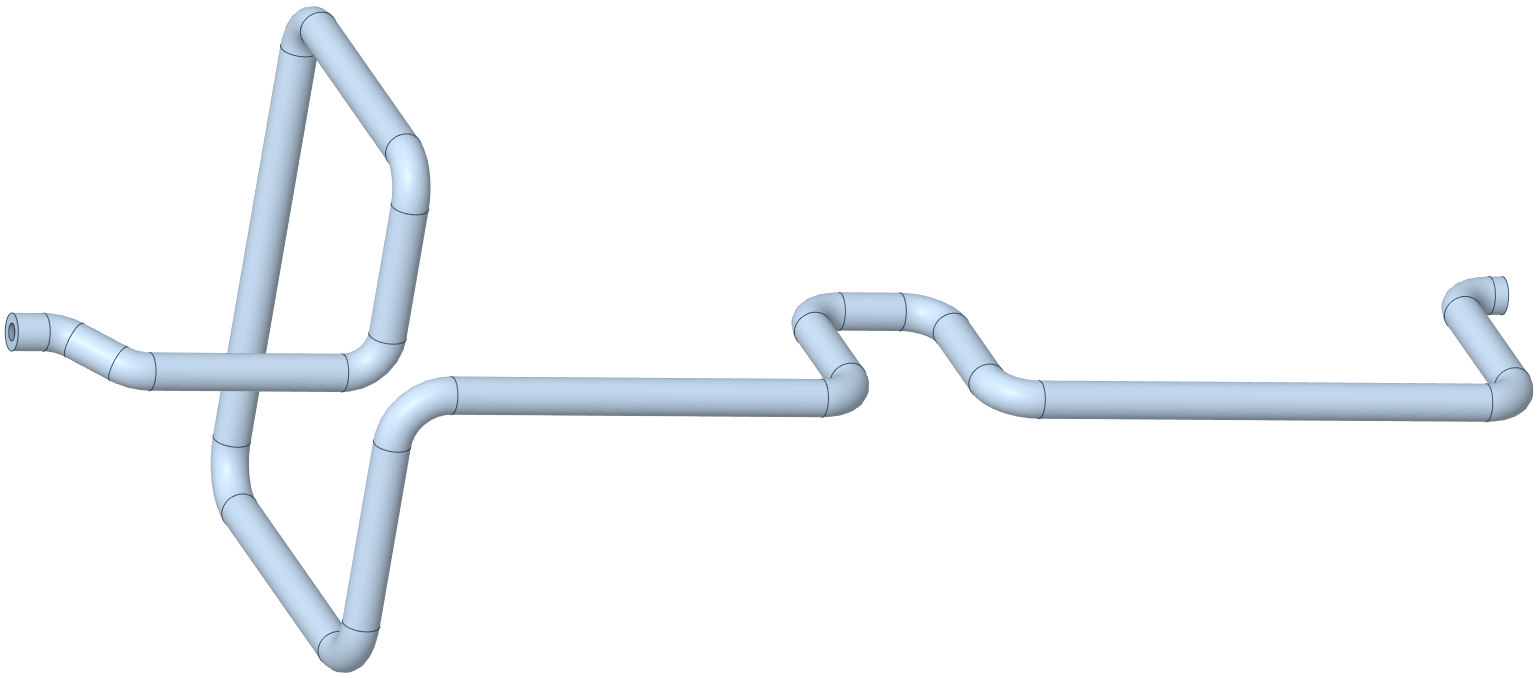
\includegraphics[width=.75\linewidth]{figures/issues_pipe_torus_a.png}
				\caption{}
				\label{fig:a}
			\end{subfigure}%
			\begin{subfigure}{.5\textwidth}
				\centering
				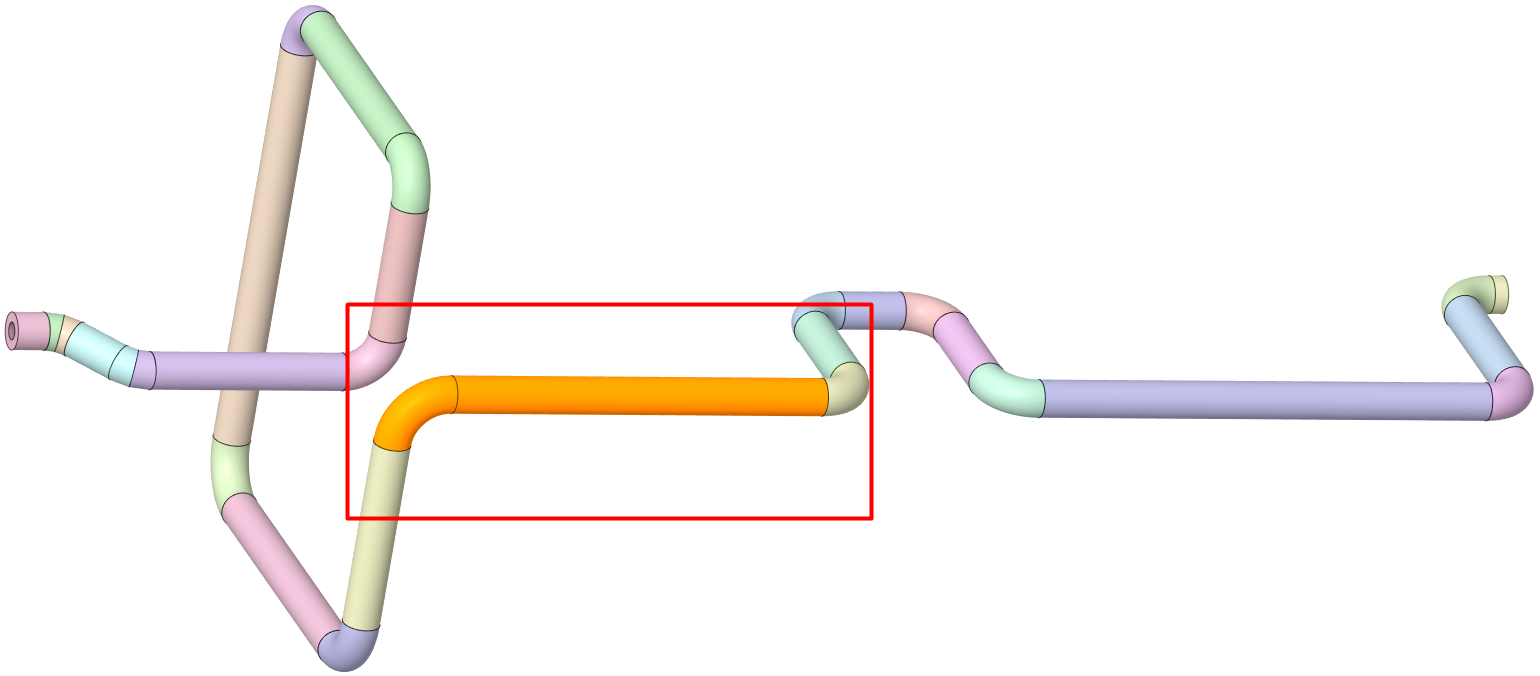
\includegraphics[width=.75\linewidth]{figures/issues_pipe_torus_b.png}
				\caption{}
				\label{fig:b}
			\end{subfigure}
			\caption{(a) Original Pipe in CAD and (b) McCAD Decomposed Pipe}
			\label{fig:McCAD Decomposed Pipe}
		\end{figure}
	\end{itemize}
	\item \textbf{Hollow solids}:
	\begin{itemize}
		\item \emph{description}: while not posing a problem for the decomposition algorithm, hollow solids pose a challenge to the run time and size of the resulting STEP file(s). Figure (\ref{fig:Hollow Solid}) shows a pipe support structure. The structure is made primarily from planar surfaces and is hollow from the inside. Processing the solid as is in McCAD would take up some time and would result in a large STEP file. As a general rule: if McCAD took more than few minutes to decompose a planar surface then maybe a manual intervention on the user side is needed. This can be achieved by manually decomposing the solid into smaller pieces then run McCAD on those subsolids.
		\item \emph{solution}: aide the decomposition by manually cut the hollow solid into three or four smaller sections which can then be processed in a reasonable time in McCAD.  
		\begin{figure}[h!]
			\centering
			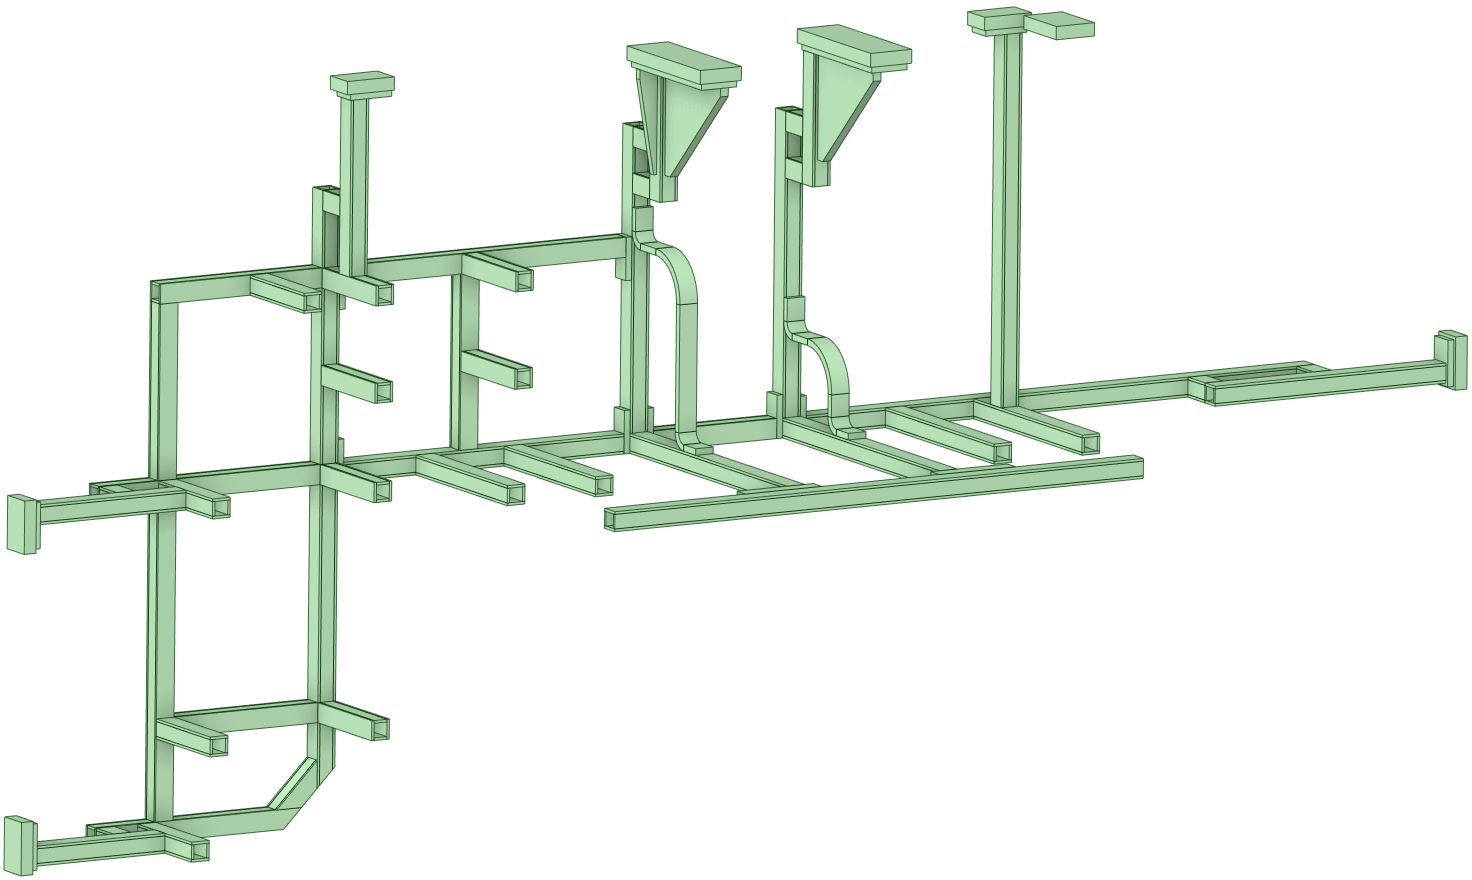
\includegraphics[scale=0.35]{figures/issues_Hollow.png}
			\caption{Coordinate System of a Solid in SpaceClaim}
			\label{fig:Hollow Solid}
		\end{figure}
	\end{itemize}
    \item \textbf{Solid names}:
    \begin{itemize}
    	\item \emph{description}: when running decomposition solid names are retrieved from component names in the input STEP file. When saving the decomposed solids to STEP files, the names appear only on the assembly level while components take the name "COMPOUND". This is due to the difficulty to give names to components in the STEP writer in OCCT.
    	\item \emph{solution}: loading the decomposed STEP files into a CAD software and manually changing the component names will alleviate such an issue and will result in actual component names appearing in cell cards in the generated MC file.  
    \end{itemize} 
\end{itemize}
\subsection{Conversion}
None thus far!

% -------------------------------------------------------------------------------------
% Theory of McCAD Conversion
% -------------------------------------------------------------------------------------
\section{Theory of McCAD Conversion} \label{sec:Theory of McCAD Conversion}
A comprehensive discussion on the inner workings of McCAD algorithms/classes for developers. Coming soon ...
\subsection{Decomposition}
\subsection{Conversion}
\newpage
% -------------------------------------------------------------------------------------
% REFERENCES
% -------------------------------------------------------------------------------------
%\bibliography{}

% -------------------------------------------------------------------------------------
% END DOCUMENT
% -------------------------------------------------------------------------------------
\end{document}